\chapter{Základné triky v LaTeX}
\label{jablka}

% Toto je komentár

Úloha tejto kapitoly je poukázať na niektoré základné triky v LaTeX pri písaní záverečnej práci. Vygenerované PDF-čko spolu so zdrojovým kódom by mali slúžiť ako návod na písanie dokumentu.


\section{Vymenovanie, číslovanie}

Neusporiadané vymenovanie môžeme v prostredí \LaTeX robiť nasledovne:
\begin{itemize}
\item Prvý bod,
\item druhý bod,
\item posledný bod.
\end{itemize}
Samozrejme môžeme používať aj podúrovňe, teda
\begin{itemize}
\item Prvý bod,
\item \begin{itemize}
\item Janko,
\item Ferko,
\item Jožko.
\end{itemize}
\item posledný bod.
\end{itemize}

Očíslované, usporiadané vymenovanie môžeme urobiť nasledovne:
\begin{enumerate}
  \item Voľba triedy operátorov $S$, na ktorej sa hľadá vlastné riešenie. Určenie triedy závisí predovšetkým od objemu apriórnej informácie a znalostí o objekte, musí však rešpektovať ciele a požiadavky syntézy riadenia a ekonomické otázky spojené s identifikáciou.
  \item Voľba vhodnej stratovej funkcie a na jej báze definovanej účelovej funkcie. Najčastejšie sú používané kvadratické účelové funkcie.
  \item Výber vhodného algoritmu pre riešenie úlohy identifikácie, t.j. optimalizačnej úlohy.
\end{enumerate}


\section{Obrázky}

Obrázky môžeme dávať do textu nasledovne. A potom jednoducho môžeme odvolať na obrázok pomocou Obr. \ref{OBRAZOK 1.1}.
%************ OBRAZOK **************
\begin{figure}[!tbh]
\centering
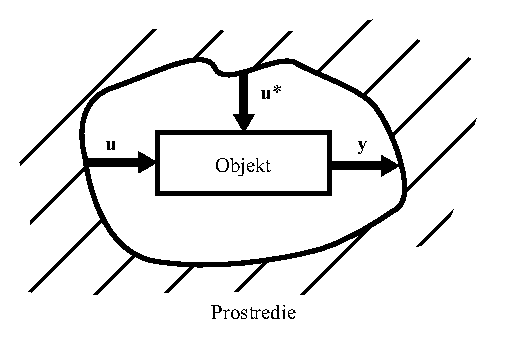
\includegraphics[width=80mm]{obr/OBRAZOK1_1.eps}
\caption{Stručný popis obrázku.}\label{OBRAZOK 1.1}
\end{figure}
%************ KONIEC **************
Nezabudnime, že popis obrázku je ukončený bodkou.

Na začiatku vety vypýšeme slovo Obrázok, kým všade inde používame skratku Obr.

\subsection{Formát obrázkov}

Pre ukladanie a zobrazenie obrázkov používame nasledovné súborové formáty:
\begin{itemize}
\item *.eps pre vektorovú grafiku (grafy, ilustrácie, priebehy)
\item *.png na screenshoty a
\item *.jpg na rasterovú grafiku (fotografie).
\end{itemize}

\subsection{Obrázky z Matlabu}

Z Matlabu exportujeme obrázky do formátu *.eps.

\section{Odvolávky na časti práce}
\label{hrusky}

Kapitolu, podkapitolu alebo podobné veci označíme príkazom "label", a nasledovne na nich odvoláme príkazom "ref". Napríklad v Kap. \ref{jablka} sme odvodili\ldots. 
Na začiatku vety vypýšeme slovo Kapitola, kým všade inde používame skratku Kap. Podkapitoly a pod-podkapitoly v odvolávkach nerozlišujeme, na štruktúru dokumentu používame vždy Kap.

\section{Matematika}

Vzorce môžeme podľa potreby priamo písať do textu, napríklad: Číselná postupnosť - množina čísel $\vec{R} \{a_m, a_{m+1}, ...\}
= \{a_m\}_{m = n}^\infty$, respektíve to očíslovať a písať do samostatného riadku napríklad pomocou
  \begin{align}
  \label{mojarovnica}
    E_0 &= mc^2                              \\
    E &= \frac{mc^2}{\sqrt{1-\frac{v^2}{c^2}}}
  \end{align}
kde potom môžeme odvolávať na rovnicu pomocou Rov. \eqref{mojarovnica}. Pozor na to, že odkaz na čísla rovnice je zahrnutá v zátvorkách, to platí iba na rovnice, nie pre obrázky, tabuľky a štruktúru dokumentu. Namiesto príkazu align, môžeme používať aj eqnarray.

Na začiatku vety vypýšeme slovo Rovnica, kým všade inde používame skratku Rov.

\section{Počítačový program}

Počítačový program môžeme jednoducho vložiť do textu pomocou
\lstset{language=exMatlab}
\begin{lstlisting}
N=1024;              % Pocet vzoriek
f1=1;                % Frekvencia harmonickeho signalu
FS=200;              % Frekvencia vzorkovania
n=0:N-1;             % Poradove cisla vzorky
x=sin(2*pi*f1*n/FS); % Generujeme signal, x(n)
[Rxx,Tau]=xcorr(x);  % Odhad autokorelacnej funkcie
\end{lstlisting}
Jazyk programu vieme určiť my, napríklad Matlab tu je rozšírený o extra príkazy.


\section{Tabuľky}

Toto je príklad tabuľky:
\begin{table}[!h]
\centering
\caption{Zoradenie metód na základe objemu apriórnych znalostí}
\begin{tabular}{ |l|c|c|c| }
  \hline
  \parbox[c]{3.5cm}{Metóda} & Kovariancia & \parbox[c]{3cm}{Hustota\\pravdepodobnosti}& Apriórna hustota\\ [0.2cm] \hline
  \parbox[c]{3.5cm}{Najmenšie štvorce} & Nie & Nie & Nie \\ [0.2cm] \hline
  \parbox[c]{3.5cm}{Najmenšie štvorce,\\Markov odhad}& Áno & Nie & Nie \\ [0.2cm]   \hline
  \parbox[c]{3.5cm}{Maximálna\\vierohodnosť}& Áno & Áno & Nie \\ [0.2cm] \hline
  \parbox[c]{3.5cm}{Bayesovské metódy} & Áno & Áno & Áno \\ [0.2cm] \hline
\end{tabular}
    \label{TABULKA_3_1}
\end{table}

Na tabuľky taktiež môžeme odvolávať pomocou Tab. \ref{TABULKA_3_1}. Tabuľky taktiež majú popis, dávame to nad tabuľkou. 

Na začiatku vety vypýšeme slovo Tabuľka, kým všade inde používame skratku Tab.

\section{Fyzykálne jednotky}

Fyzikálne jednotky oddelujeme medzerou od čísla a píšeme nezmeneným typom písma, t.j. nepoužívame šikmé písmo. Používame medzinárodne známe a akceptované jednotky a skratky jednotiek. Správne je teda 10 V, nesprávne je to 10V, 10 Volt, 10 \emph{V}. 


\section{Bibliografické citácie}

Citovať môžeme nasledovne \cite{Eykhoff84}. Ak chceme citovať viacero autorov, tak môžeme to robiť naraz \cite{Fontes00,Eykhoff84}. Databazu citovanych dokumentov piseme do suboru *.bib. Všetky typy dokumentov (kniha, článok etc.) má svoju vlastnú kategóriu. Autora publikácie môžeme aj napísať, napríklad že v práci Qin a Badgwell \cite{Qin99} dokázali že. Citácia je súčasťou vety, môžeme to kombinovať do vety \cite{Karny80} alebo dávať pred bodkou na koniec \cite{Far90}.

\section{Príklad}

Ak chceme uviesť inštrukčný príklad, potom na to máme prostredie
\begin{exmp}
Jožko má 5 melónov, vypočítajte hmotnosť Slnka.
\end{exmp}
kde príklad je ukončený znamienkom QED (štvorec).





